\documentclass{beamer}
\usetheme{Warsaw}
\usecolortheme{beaver}
\title[Bias, Variance and Parsimony in Regression Analysis]{Bias, Variance and Parsimony in Regression Analysis\\ECS 256 Winter 2014}
\author[Prof. Norm Matloff Winter 2014]{
Christopher Patton, \texttt{cjpatton@ucdavis.edu}\\
Alex Rumbaugh, \texttt{aprumbaugh@ucdavis.edu}\\
Thomas Provan,\texttt{tcprovan@ucdavis.edu}\\
Olga Prilepova, \texttt{prilepova@gmail.com}\\
John Chen, \texttt{jhochen@ucdavis.edu}}
\institute{ECS 256, Winter 2014\\ \Large{UC Davis}}
\date{March 12, 2014}
\begin{document}

\begin{frame}
\titlepage
\end{frame}


\begin{frame}{Introduction}
%This is the introduction.
\end{frame}

% Alex's Section -----------------------------------------------------------------
\author[Alex Rumbaugh]{C. Patton, A. Rumbaugh, T. Provan, O. Prilepova, J. Chen}
\begin{frame}
    \frametitle{California Housing Data}
	\begin{itemize}
		\item {Derived from 1990 Census}
		\item {Response Variable: median house value}
		\item {Predictor Variables: median income, housing median age, total rooms, total bedrooms, population, households, latitude, and longitude}
	\end{itemize}
\end{frame}

\begin{frame}
    \frametitle{Parsimony}
	\begin{tabular}{ | c | p{2.7cm} | p{2.7cm} | c  |} 
\hline
Method&Parsimony (k=0.01) & Parsimony (k=0.05) & Sig Test \\
\hline
Columns  Deleted& Total Rooms \newline Total Bedrooms & Total Rooms \newline Total Bedrooms \newline Median Age & None \\
\hline
Adjusted $R^2$ & 0.6321316 & 0.6218261 & 0.6369649 \\
\hline
\end{tabular}
\end{frame}

\begin{frame}[fragile]
    \frametitle{Regression Coefficients}
\begin{verbatim}
Coefficients:
                 Estimate Std. Error t value Pr(>|t|)    
(Intercept)    -3.594e+06  6.254e+04 -57.468  < 2e-16 ***
Median.Income   4.025e+04  3.351e+02 120.123  < 2e-16 ***
Median.Age      1.156e+03  4.317e+01  26.787  < 2e-16 ***
Total.Rooms    -8.182e+00  7.881e-01 -10.381  < 2e-16 ***
Total.Bedrooms  1.134e+02  6.902e+00  16.432  < 2e-16 ***
Population     -3.854e+01  1.079e+00 -35.716  < 2e-16 ***
Households      4.831e+01  7.515e+00   6.429 1.32e-10 ***
Latitude       -4.258e+04  6.733e+02 -63.240  < 2e-16 ***
Longitude      -4.282e+04  7.130e+02 -60.061  < 2e-16 ***
\end{verbatim}
\end{frame}

\begin{frame}[fragile]
    \frametitle{Latitude \& Longitude}
\begin{verbatim}
	Latitude       -4.258e+04  6.733e+02 -63.240  < 2e-16 ***
	Longitude      -4.282e+04  7.130e+02 -60.061  < 2e-16 ***
\end{verbatim}
\begin{itemize}
\item "Center of Gravity"
\item Avoid Overfitting
\end{itemize}
	
\end{frame}

\begin{frame}[fragile]
    \frametitle{Understanding}
	\begin{verbatim}
Coefficients:
                Estimate Std. Error t value Pr(>|t|)    
(Intercept)   -32165.268   2167.358  -14.84   <2e-16 ***
Median.Income  43094.918    284.263  151.60   <2e-16 ***
Median.Age      2000.544     45.080   44.38   <2e-16 ***
Population       -43.045      1.127  -38.20   <2e-16 ***
Households       152.700      3.344   45.66   <2e-16 ***
\end{verbatim}
\end{frame}

\begin{frame}
	\begin{figure}
 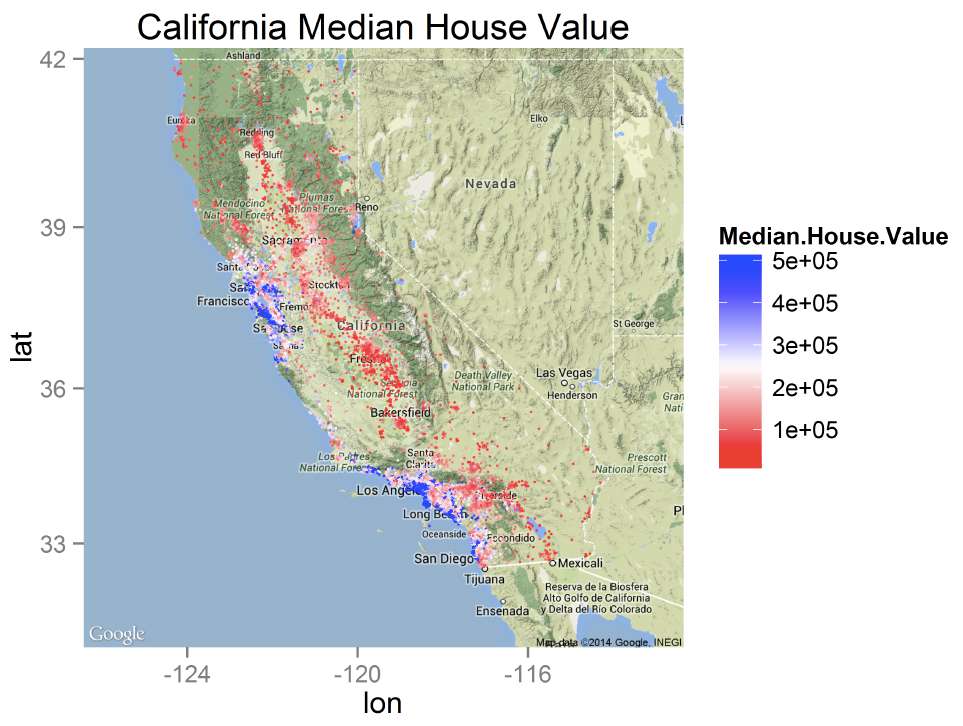
\includegraphics[scale=0.3]{figures/california.png}
\end{figure}
\end{frame}

\begin{frame}
	\begin{figure}
 \includegraphics[scale=0.3]{figures/losangeles.png}
\end{figure}
\end{frame}

\begin{frame}
	\begin{figure}
 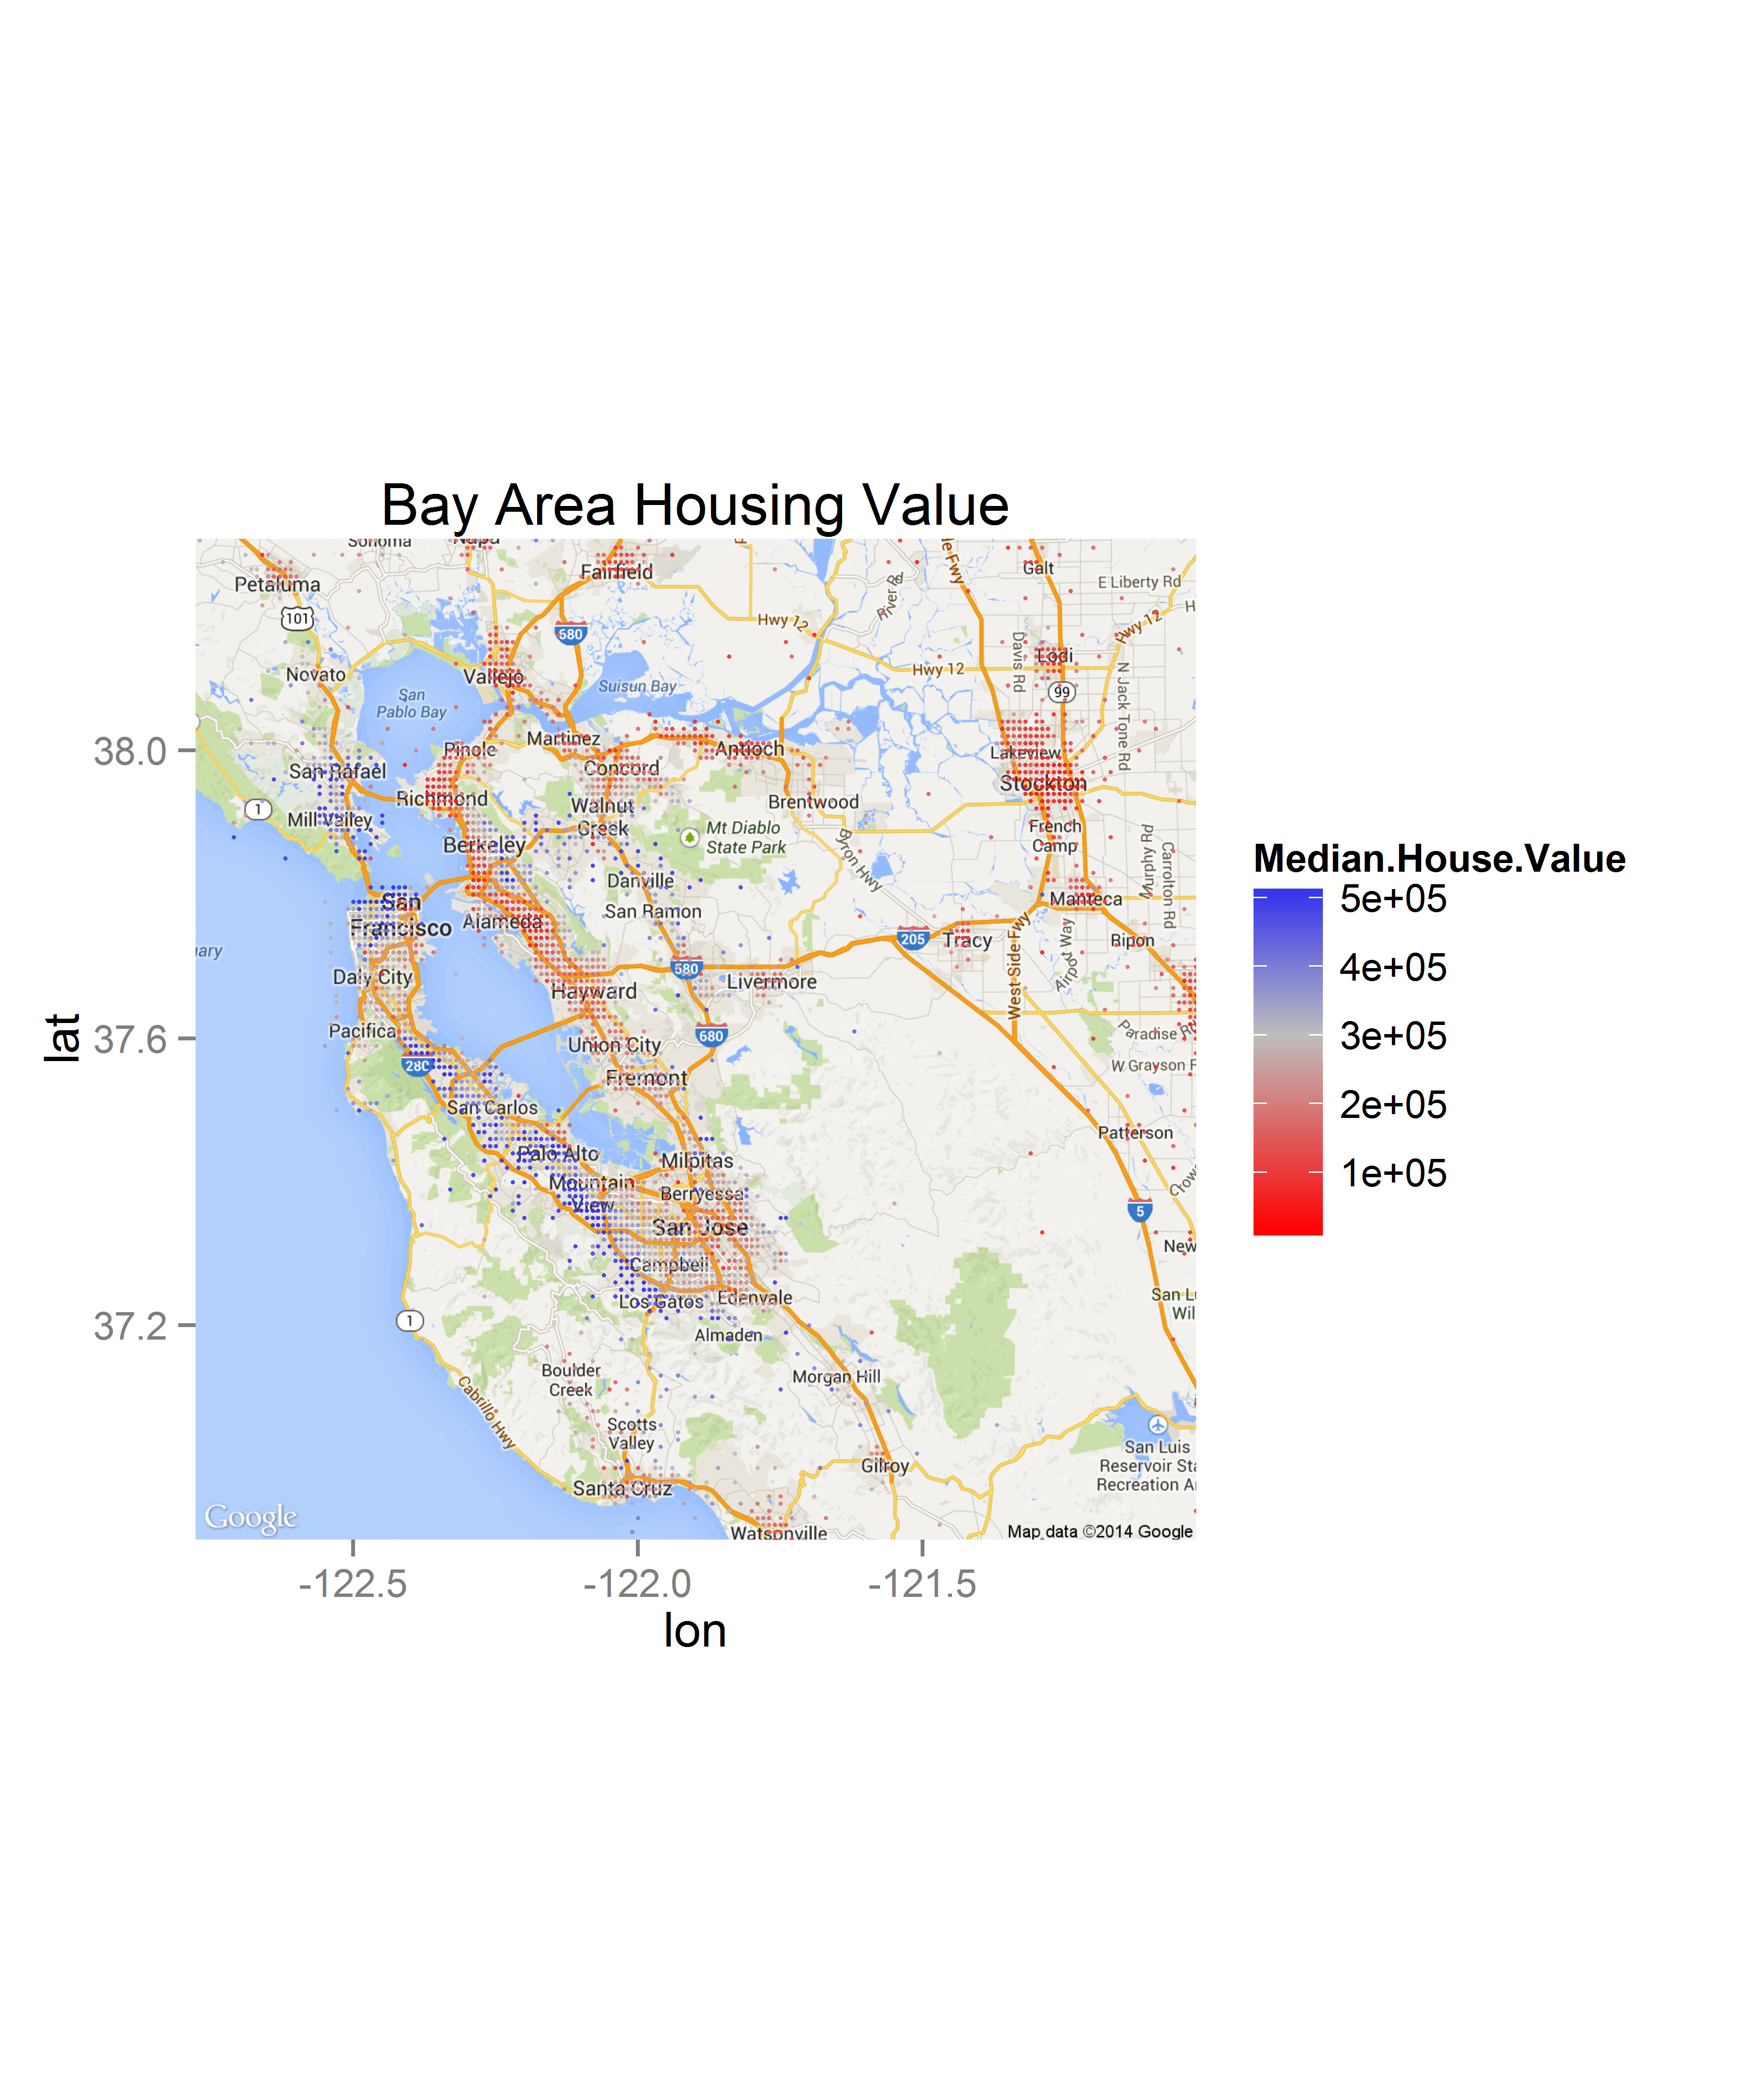
\includegraphics[scale=0.3]{figures/bayarea.png}
\end{figure}
\end{frame}

% End Alex's Section--------------------------------------------------------------

% Olga's Section--------------------------------------------------------------
\author[Olga Prilepova]{C. Patton, A. Rumbaugh, T. Provan, O. Prilepova, J. Chen}

\begin{frame}
\frametitle{Census Based on 1994}
\end{frame}

\begin{frame}
\frametitle{Age}
\end{frame}

\begin{frame}
\frametitle{}

\begin{figure}
 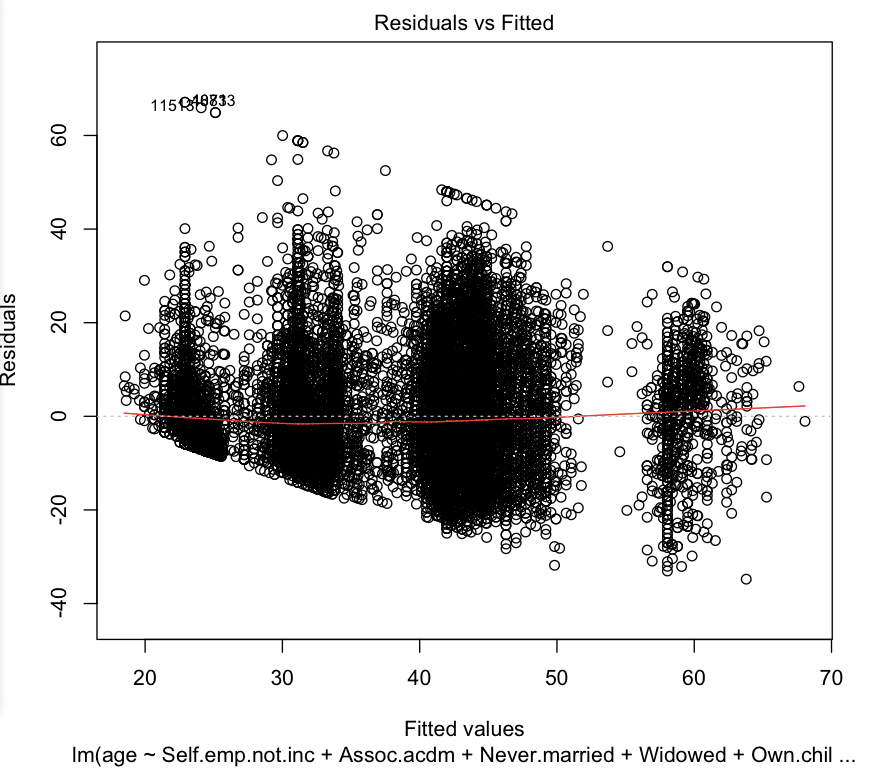
\includegraphics[scale=0.3]{figures/ageResidCensus.png}
 \label{fig:ageResidCensus}
\end{figure}
 
\end{frame}

\begin{frame}
\frametitle{Census Based on 1994}
% Census Sex Coefficients
\end{frame}

\begin{frame}
\frametitle{Census Based on 1994}
% Census Salary Coefficients
\end{frame}

\begin{frame}
%Picture of predicted vs actual age
\begin{figure}
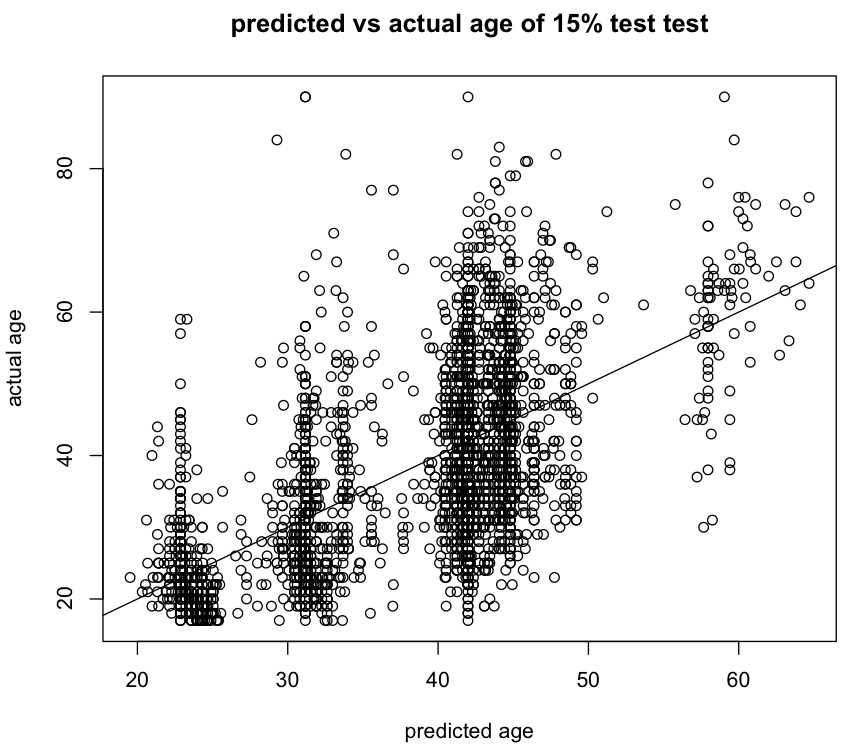
\includegraphics[scale=0.3]{figures/predVsActualCensus.png}
\label{fig:predVsActualCensus}
\end{figure}
\end{frame}

\begin{frame}
%Picture of predicted vs actual age

\begin{figure}
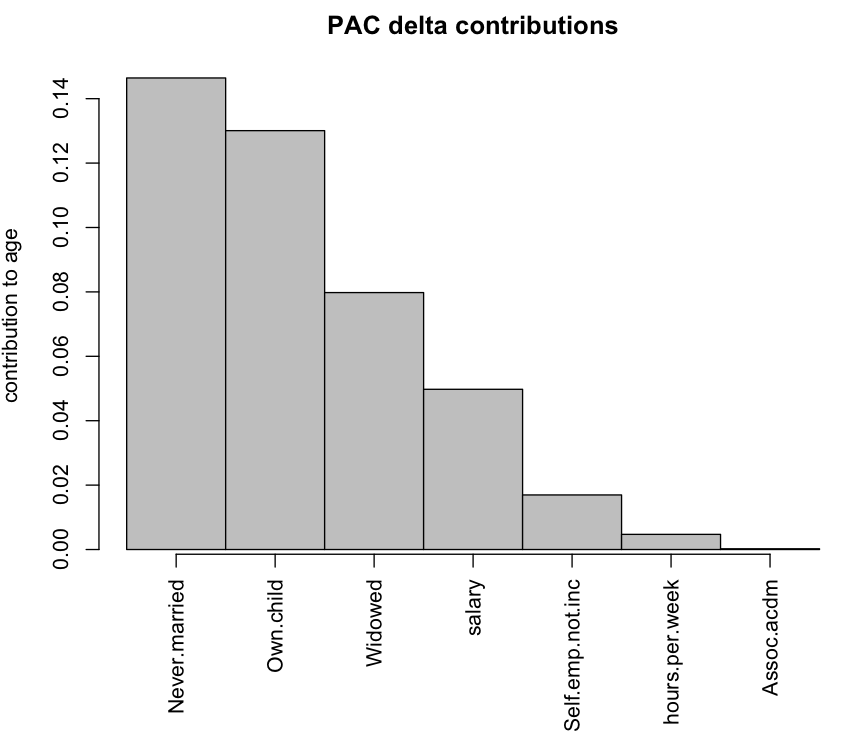
\includegraphics[scale=0.3]{figures/ageContrib.png}
\caption{}
 \label{fig:ageContrib}
\end{figure}

\end{frame}
% End Olga's Section--------------------------------------------------------------

% Begin Chris' Section--------------------------------------------------------------
\author[Christopher Patton]{C. Patton, A. Rumbaugh, T. Provan, O. Prilepova, J. Chen}

\begin{frame}
\frametitle{}
%Slide 1
\end{frame}

\begin{frame}
\frametitle{}
%Slide 2
\end{frame}

\begin{frame}
\frametitle{}
%Slide 3
\end{frame}

\begin{frame}
\frametitle{}
%Slide 4
\end{frame}

\begin{frame}
\frametitle{}
%Slide 5
\end{frame}

% End Chris' Section--------------------------------------------------------------
% Thomas' Section--------------------------------------------------------------

% Theme: Problem 2b Parsimony on Simulated Data
\author[Thomas Provan]{C. Patton, A. Rumbaugh, T. Provan, O. Prilepova, J. Chen}

\begin{frame}
\frametitle{Testing Parsimony on Simulated Data}
%Slide 1

Predictors: $X = X_1,..., X_10$

Response: $Y$ drawn from $U(m_{Y;X}(t) - 1, m_{Y;X}(t) + 1)$

\vspace{1 mm}

\hspace{8 mm} where $m_{Y,X}(t) = t_1 + t_2 + t_3 + 0.1t_4 + 0.01t_5$


\end{frame}

\begin{frame}
\frametitle{Testing Parsimony on Simulated Data}
%Slide 2

\begin{tabular}{| l  r | c | c | c |}

\hline

	&&	prsm(k=0.01)&	prsm(k=0.05)&	sig test	\\
\hline

n=100&	Run 1&	$X_1 ,X_2, X_3, X_9$&	$X_1, X_2, X_3$&		$X_1, X_2, X_3$	\\
	&	Run 2&	$X_1, X_2, X_3$&		$X_1, X_2, X_3$&		$X_1, X_2, X_3$	\\
	&	Run 3&	$X_1, X_2, X_3$&		$X_1, X_2, X_3$&		$X_1, X_2, X_3$	\\

\hline

n=1000&	Run 1&	$X_1, X_2, X_3$&		$X_1, X_2, X_3$&		$X_1, X_2, X_3, X_4$	\\
	&	Run 2&	$X_1, X_2, X_3$&		$X_1, X_2, X_3$&		$X_1, X_2, X_3$		\\
	&	Run 3&	$X_1, X_2, X_3$&		$X_1, X_2, X_3$&		$X_1, X_2, X_3$		\\
	
\hline
			
n=10K&	Run 1&	$X_1, X_2, X_3$&		$X_1, X_2, X_3$&		$X_1, X_2, X_3, X_4$		\\
	&	Run 2&	$X_1, X_2, X_3$&		$X_1, X_2, X_3$&		$X_1, X_2, X_3, X_4$		\\
	&	Run 3&	$X_1, X_2, X_3$&		$X_1, X_2, X_3$&		$X_1, X_2, X_3, X_4, X_9$		\\

\hline
			
n=100K&	Run 1&	$X_1, X_2, X_3$&		$X_1, X_2, X_3$&		$X_1, X_2, X_3, X_4$		\\
	&	Run 2&	$X_1, X_2, X_3$&		$X_1, X_2, X_3$&		$X_1, X_2, X_3, X_4, X_9$		\\
	&	Run 3&	$X_1, X_2, X_3$&		$X_1, X_2, X_3$&		$X_1, X_2, X_3, X_4, X_9$		\\

\hline

\end{tabular}


\end{frame}

\begin{frame}[shrink=8]
\center
\frametitle{Testing Parsimony on Simulated Data}

\begin{tabular}{| l | c | c | c | c | c | c | c | c | c | c |}



\hline
\textbf{k=0.01}&	$X_1$&	$X_2$&	$X_3$&	$X_4$&	$X_5$&	$X_6$&	$X_7$&	$X_8$&	$X_9$&	$X_{10}$\\
\hline
N = 100&			1&	1&	1&	0.24&	0.11&	0.14&	0.21&	0.22&	0.26&	0.28 	\\
N = 1000&			1&	1&	1&	0.08&	0&	0&	0&	0&	0&	0	\\
N = 10K&			1&	1&	1&	0&	0&	0&	0&	0&	0&	0	\\
N = 100K&			1&	1&	1&	0&	0&	0&	0&	0&	0&	0	\\
N = 1M&			1&	1&	1&	0&	0&	0&	0&	0&	0&	0	\\
\hline		

\\
								
									\\		
\hline					
\textbf{k=0.05}&	$X_1$&	$X_2$&	$X_3$&	$X_4$&	$X_5$&	$X_6$&	$X_7$&	$X_8$&	$X_9$&	$X_{10}$\\
\hline
N = 100&			1&	1&	0.99&	0.1&	0.02&	0.05&	0.04&	0.03&	0.07&	0.02	\\
N = 1000&			1&	1&	1&	0&	0&	0&	0&	0&	0&	0	\\
N = 10K&			1&	1&	1&	0&	0&	0&	0&	0&	0&	0	\\
N = 100K&			1&	1&	1&	0&	0&	0&	0&	0&	0&	0	\\
N = 1M&			1&	1&	1&	0&	0&	0&	0&	0&	0&	0	\\
\hline


\end{tabular}


\end{frame}

\begin{frame}[shrink=8]
\center
\frametitle{Testing Parsimony on Simulated Data}
\begin{tabular}{| l | c | c | c | c | c | c | c | c | c | c |}
		
\hline
\textbf{Sig Test}&	$X_1$&	$X_2$&	$X_3$&	$X_4$&	$X_5$&	$X_6$&	$X_7$&	$X_8$&	$X_9$&	$X_{10}$\\
\hline
N = 100&		1&	1&	1&	0.14&	0.03&	0.05&	0.05&	0.03&	0.09&	0.04	\\
N = 1000&		1&	1&	1&	0.31&	0.02&	0.05&	0.05&	0.05&	0.02&	0.04	\\
N = 10K&		1&	1&	1&	1&	0.04&	0.01&	0.07&	0.07&	0.03&	0.06	\\
N = 100K&		1&	1&	1&	1&	0.35&	0.06&	0.09&	0.03&	0.05&	0.03	\\
N = 1M&		1&	1&	1&	1&	1&	0.05&	0.03&	0.08&	0.02&	0.03	\\
\hline
\end{tabular}
\end{frame}


% End Thomas' Section--------------------------------------------------------------
% John's Section--------------------------------------------------------------

\author[John Chen]{C. Patton, A. Rumbaugh, T. Provan, O. Prilepova, J. Chen}
% Theme: Automobile Analysis & Accurate Predictors
\begin{frame}
\frametitle{Small N, Large P}
%Slide 1
\end{frame}

\begin{frame}
\frametitle{Parsimony: Automobile Prices}
%Slide 2
\end{frame}

\begin{frame}[fragile]
\frametitle{Significance Testing: Auto Prices}
\texttt{Summary of Significance Testing:}\\
\tiny{ 
\begin{verbatim}
(Intercept)     -4.234e+04  1.125e+04  -3.764 0.000229 ***
bmw              9.290e+03  8.611e+02  10.788  < 2e-16 ***
dodge           -1.504e+03  8.532e+02  -1.762 0.079785 .  
`mercedes-benz`  6.644e+03  1.003e+03   6.625 4.17e-10 ***
mitsubishi      -2.628e+03  7.331e+02  -3.585 0.000438 ***
plymouth        -1.628e+03  8.881e+02  -1.833 0.068485 .  
porsche          4.053e+03  2.238e+03   1.811 0.071936 .  
saab             2.413e+03  1.028e+03   2.347 0.020043 *  
std             -1.109e+03  5.129e+02  -2.162 0.031973 *  
front           -1.275e+04  2.663e+03  -4.785 3.63e-06 ***
wheel.base       1.141e+02  7.390e+01   1.544 0.124355    
length          -7.918e+01  4.225e+01  -1.874 0.062586 .  
width            7.652e+02  2.029e+02   3.772 0.000222 ***
height          -1.377e+02  1.164e+02  -1.183 0.238332    
curb.weight      3.781e+00  1.118e+00   3.381 0.000890 ***
dohc             1.569e+03  8.067e+02   1.944 0.053451 .  
ohc              8.531e+02  4.575e+02   1.865 0.063911 .  
engine.size      7.733e+01  1.035e+01   7.470 3.74e-12 ***
peak.rpm         1.522e+00  3.938e-01   3.864 0.000157 ***
---
Multiple R-squared:  0.9373,	Adjusted R-squared:  0.9308 
F-statistic: 144.5 on 18 and 174 DF,  p-value: < 2.2e-16  
\end{verbatim}
}
\end{frame}

\begin{frame}
\frametitle{Parsimony: Auto Safety}
%Slide 4
\end{frame}

\begin{frame}[fragile]
\frametitle{Significance Testing: Auto Safety}

\texttt{Summary of Significance Testing:}\\
\tiny{
\begin{verbatim}
Coefficients:
              stimate Std. Error z value Pr(>|z|)    
(Intercept)    E 2.5122     1.1216   2.240  0.02510 *  
audi           20.3574  2027.3521   0.010  0.99199    
saab           17.7446  1985.9220   0.009  0.99287    
volkswagen      1.8112     0.9634   1.880  0.06011 .  
diesel         -2.0155     1.2716  -1.585  0.11297    
std            -0.4196     1.0765  -0.390  0.69668    
`four-doors`   -5.9725     1.1293  -5.288 1.23e-07 ***
`4wd`          -0.1377     2.1849  -0.063  0.94976    
fwd             3.3028     1.1093   2.977  0.00291 ** 
`1bbl`         -4.4965     1.4035  -3.204  0.00136 ** 
---
Null deviance: 266.06  on 192  degrees of freedom
Residual deviance: 110.24  on 183  degrees of freedom
AIC: 130.24
\end{verbatim}
}
\end{frame}
% End John's Section--------------------------------------------------------------

\author[Q \& A]{
Christopher Patton, \texttt{cjpatton@ucdavis.edu}\\
Alex Rumbaugh, \texttt{aprumbaugh@ucdavis.edu}\\
Thomas Provan,\texttt{tcprovan@ucdavis.edu}\\
Olga Prilepova, \texttt{prilepova@gmail.com}\\
John Chen, \texttt{jhochen@ucdavis.edu}}

\begin{frame}
\titlepage
\end{frame}

\end{document}